\section{Safety}

In this section, building off the definition provided in~\cite{DBLP:journals/corr/HuangKWW16}, we provide a formal definition of the vulnerability to adversarial input of a mealy machine where the transition actions are neural networks.
We then show how by decomposing a larger neural network into an automata of smaller neural networks, we can reduce the overall vulnerability of the system.
Relying on the structure of the automata connecting the network, we can provide formal proofs activation periods of each individual network and demonstrate that adversarial inputs are less likely to be acted upon within a given time frame.

Previous work gives a definition of safety with respect to small perturbations in input~\cite{DBLP:journals/corr/HuangKWW16}.
``We define a network decision to be \textit{safe} for input x and region $\mu$ with respect to the set of manipulations $\delta$ if applying the manipulations on x will not result in a class change for $\mu$.''
Since we focus on building neural networks that are resilient to the sensor spoofing attacks uniquely possible in cyber physical systems, we require a slightly different definition of safety.

We consider spoofing attacks on cyber physical systems which use some neural network architecture in their controller.
The controller processes multiple streams of input (\inputSig{0}{t},\inputSig{1}{t}, ..., \inputSig{n}{t}), and produces output streams (\outputSig{0}{t}, \outputSig{1}{t}, ..., \outputSig{m}{t}) over infinite time points $t$.
In a spoofing attack, an attacker controls a set of the input streams $atk \subseteq \inputSig{0...n}{t}$ during times steps $\atkBegin<t<\atkBegin+\atkLength$.
The goal of this adversary to alter the network's behaviour (\outputSig{0...n}{t}) such that the system reaches an unsafe state.
We will define an unsafe state with respect to an abstraction on the dynamics of the system, captured by a hybrid automata model of the system.
We define a network to be \textit{resilient} if the controller stays in the safe region.


%Generally, we can expect $n>\atkLength$, as an adversary will push the system into a state (a space of input stream values) from which it will take some time to recover.
\subsection{Attacking the gear train}

To represent a gear train controller that is vulnerable to a spoofing attack, we extend Fig~\ref{fig:full} with the new predicate \isUnderAttack to act as an oracle in the model to tell if the system is under attack.
As shown in Fig.~\ref{fig:fullAtk}, when under attack, the \fullNN will receive an attacked input stream value ($speed_{ATK}$).

\begin{figure}[h!]
\centering
\begin{tikzpicture}[shorten >=1pt,node distance=2.8cm,on grid]
  \node[state]   (q_0)                {$q_0$};
  \path[->] (q_0) 
		  edge [loop above]   node  [above,align=center]         {$\neg\isUnderAttack,$\\$ \fullNN$} ();
  \path[->] (q_0) 
		  edge [loop below]   node  [below,align=center]         {$\isUnderAttack,$\\$ \fullNNAtk$} ();
\end{tikzpicture}
\caption{A mealy machine of a single monolithic neural network that is vulnerable to a spoofing attack}
\label{fig:fullAtk}
\end{figure}

We express the safety of the system as reachability on a hybrid automata.
This requires spliting the state $q_0$ to capture the two different dynamics of the systems according to the inputs streams.
The inuition is that when under attack, the dynamics of the system approach some unsafe space, whereas during normal operations, the controller brings the system back into a safe space.
In the example in Fig.~\ref{fig:hybridGear}, we use a $\dot{x}$ to represent the continuous flow of the value x induced by the control mode (e.g. \fullNN).
When under attack, $x$ will flow towards an unsafe space (e.g. $x > 10$), when not under attack, the controller will push $x$ back to a safe space (e.g. $x\leq 10$)

\begin{figure}[h!]
\centering
\begin{tikzpicture}[shorten >=1pt,node distance=1.2cm,on grid]
  \node[rectangle,draw]   (q_0)                {$\dot{x} = 1$};
  \node[rectangle,draw]   (q_1) [below of=q_0] {$\dot{x} = -1$};
  \path[->] (q_0) 
		  edge [loop above]   node  [above,align=center]         {$\neg\isUnderAttack,$\\$ \fullNN$} ();
	\path[->] (q_0) edge [bend right] (q_1);
	\path[->] (q_1) edge [bend right] (q_0);
  \path[->] (q_1) 
		  edge [loop below]   node  [below,align=center]         {$\isUnderAttack,$\\$ \fullNNAtk$} ();
\end{tikzpicture}
\caption{A hybrid automata expressing the how the mode changes affect the dynamics of the system.}
\label{fig:hybridGear}
\end{figure}


\subsection{Mixture of Experts}

From a machine learning perspective, we can view this architecture as an instance of the mixture of experts architecture.
In this case, the Mealy machine acts as the \textit{Gating Network} in Fig.~\ref{fig:MOE}.
By using an explicit structure for the gating networks (as opposed to another neural network), we enable a level of legibiilty over the entire system.

\begin{figure}[h!] %[h] para here [b] para bottom [t] para top
\centering
	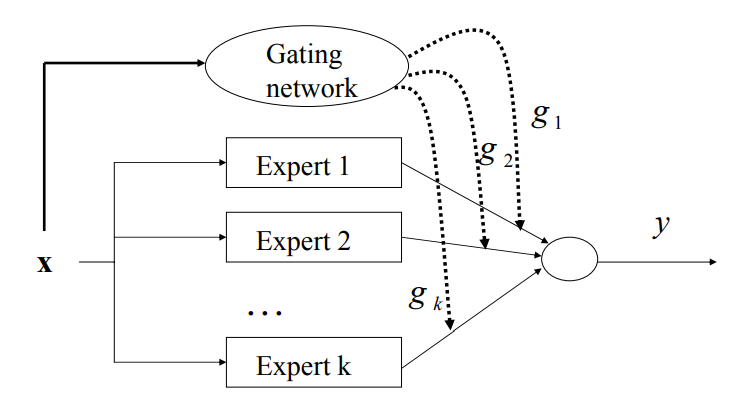
\includegraphics[width=0.49\textwidth]{MOE.png}
\caption{Mixture of experts scheme.}
\label{fig:MOE}
\end{figure}

